The network metering with Zabbix is not only used for network managing decisions. It is also possible for each user of the \textit{Smart Filesystem} to get informations concerning his created costs based on consumed energy by servers usage.

\subsection{User report generation schema}
  Reports can be read and generated via a small reporting web frontend. Involved Java classes and the overall procedure is shown in figure~\ref{akt}.

 \begin{figure}
 \centering
 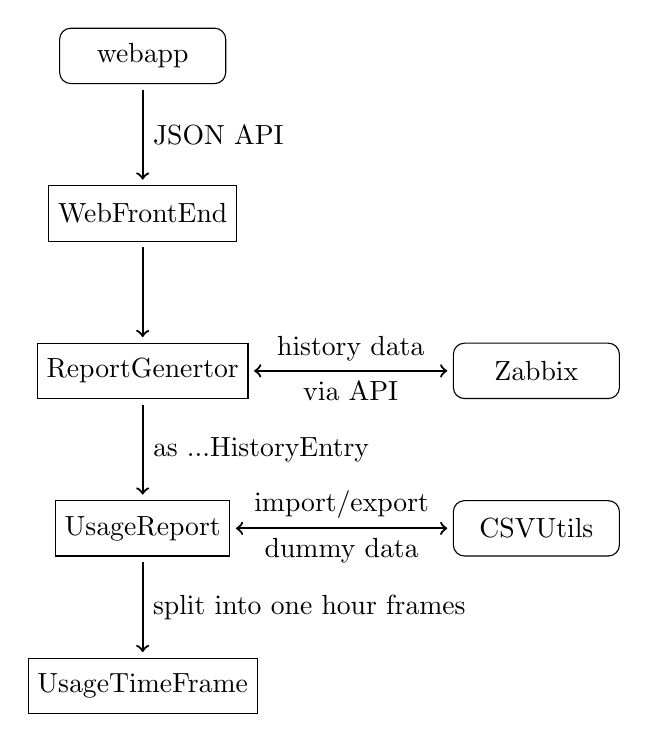
\begin{tikzpicture}
    \tikzset{
        external/.style = {
            rectangle, rounded corners, draw=black,
            minimum width=6em, minimum height=2em, text centered, node distance=5cm
        },
        internal/.style = {
            rectangle, draw=black,
            minimum width=6em, minimum height=2em, text centered, node distance=2cm
        },
        edge/.style = {
            ->, thick, shorten <= 2pt, shorten >= 2pt
        },
        dotted box/.style = {
            rectangle, draw = black, rounded corners, dashed, inner sep=3pt
        }
    };

	\node[internal] (generator) {ReportGenertor};
	\node[internal] (web) [above of = generator] {WebFrontEnd};
	\node[external, node distance = 2cm] (webapp) [above of = web] {webapp};
	\node[external] (zabbix) [right of = generator]  {Zabbix};
	\node[internal] (report) [below of = generator] {UsageReport};
	\node[external] (csv) [right of = report] {CSVUtils};
	\node[internal] (frame) [below of = report]{UsageTimeFrame};

	\draw[edge] (webapp) -- (web) node [midway, right] {JSON API};
	\draw[edge] (web) -- (generator);
	\draw[edge, <->] (generator) -- (zabbix)
		node [midway, above] {history data}
		node [midway, below] {via API};
	
	\draw[edge, <->] (report) -- (csv) 
		node [midway, above] {import/export} 
		node [midway, below] {dummy data};
	
	\draw[edge] (generator) -- (report)
		node [midway, right] {as ...HistoryEntry};
	\draw[edge] (report) -- (frame) 
		node [midway, right] {split into one hour frames};
\end{tikzpicture}
 \caption{Report generation procedure and involved Java classes}
 \label{akt}
 \end{figure}

 Reports can be generated with live data (online mode) or dumped/save as csv raw data files (offline mode). The report request goes to the "ReportGenerator" wich collects the online data via a Zabbix client instance and encapsulates them within a UsageReport. All data gets now ordered by date and splitted into usage time frames (one hour). All calculations are based and summarized on this time frames.
 
 \subsection{Calculation of the price} 
 The price calculation concept covers the power consumption of the \textit{Smart Filesystem} and does not include any maintance costs.
 Every user has to pay a part of the energy usage if the severs run in idle mode. The part depends on how much data the user has stored in the system. Moreover the user has to pay for his traffic, which normally results in a higher power usage. It should be noticed that this basic concept, which was designed by the team, can't work if just a few persons uses the system. Distributed file systems are generally made for a lot of people using them and/or a lot of data stored in this system. Our simulation was unable to test such a situation because there simply were not that much test users and our test system was comparatively small. 
 
 If we want to compute the price for each user in an hour, the first thing to do is to extend the data from Zabbix. Firstly Zabbix stores energy usage of each sever every two seconds. Secondly, if there is a traffic flow, Zabbix will store information about that every five seconds. And last but not least Zabbix stores the used data of each user if it changes. Imagine a situation where user \textit{u} transfers 100 megabytes in 10 seconds to the \textit{Asok05} server. Then the information created by Zabbix looks like table~\ref{tb1}. 
 To get clear information when a flow starts and when a flow stops, Floodlight sends at the start and the end of a flow a zero to Zabbix. Storage usage gets reported on every change by the HDFS name node.

\begin{table}
\centering
\caption{Generated data from Zabbix of user \textit{u}}
\begin{tabular}{|c|c|c|c|}
 \hline Time in $s$ & Data in $MB$ & Traffic in $MB/s$ & Energy in $W$ \\ 
  \hline 0 & 3000 & 0 & 400 \\ 
 \hline 1 & - & 10 & - \\ 
 \hline 2 & - & - & 115 \\ 
 \hline 3 & - & - & -\\ 
 \hline 4 & - & - & 430 \\ 
 \hline 5 & - & - & - \\
 \hline 6 & - & 10 & 445 \\ 
 \hline 7 & - & - & -\\ 
 \hline 8 & - & - & 445 \\ 
 \hline 9 & - & - & - \\  
 \hline 10 & - & - & 430 \\
  \hline 11 & - & 10 & - \\
 \hline 12 & 3100 & 0 & 415 \\  
 \hline 
 \end{tabular}
 \label{tb1} 
 \end{table}
 
 The initial values (0s) are based on the last known values. The given information is not enough to compute a price for each user at every second. So the next step is to complete the table by interplolating the data. For every empty energy entry the system takes the next known value. For the storage usage the system takes the last known value (if something changes, new values are present). Traffic values are represented as average over the last five seconds by floodlight and can be simply extended on the next values. After interplolating the data our table looks like table~\ref{tb2}.
 
 \begin{table}
 \centering
 \caption{Extended Data of user \textit{u}}
 \begin{tabular}{|c|c|c|c|}
  \hline Time in s & Data in $MB$ & Traffic in $MB/s$ & Energy in $W$ \\ 
   \hline 0 & 3000 & 0 & 400 \\ 
  \hline 1 & 3000 & 10 & 415 \\ 
  \hline 2 & 3000 & 10 & 415 \\ 
  \hline 3 & 3000 & 10 & 430 \\ 
  \hline 4 & 3000 & 10 & 430 \\ 
  \hline 5 & 3000 & 10 & 445 \\
  \hline 6 & 3000 & 10 & 445 \\ 
  \hline 7 & 3000 & 10 & 445 \\ 
  \hline 8 & 3000 & 10 & 445 \\ 
  \hline 9 & 3000 & 10 & 430 \\  
  \hline 10 & 3000 & 10 & 430 \\
   \hline 11 & 3000 & 10 & 415 \\
  \hline 12 & 3100 & 0 & 415 \\  
  \hline 
  \end{tabular}
  \label{tb2} 
  \end{table}
  
  This extended table will be created for each user, each server and for each time frame. If there is user data synchronization between the servers, it will identified as "internal traffic" and will be accounted for a user on the system which does the synchronization. After that, the system can compute a price for each user in each second of an hour. After that it sums up the prices and computes the mean value. Then we have the costs for each user and for each system. The last step is to sum up the mean values for each system to get the total costs for a user in an hour / time frame.
  
  Computing the price for second must be separated in two different situations. The question is: "Does a user create traffic in this second?":
  \begin{enumerate}
	\item
	If not, the system will compute the ratio of used data storage by a user compared to overall used data storage and multiplies it by the power consumption of the server in idle mode.
	\item
	If a user does create traffic it will do the same as in step one. Moreover it will compute the ratio of user traffic to all user traffic to this server and multiplies it with the needed energy in this second deducing the idle energy consumption.
  \end{enumerate}
  
  \subsection{Example}
    For instance the idle energie consumption of \textit{Asok05} is $400\ W$ and usage values are as listed in table~\ref{tb2}. Moreover say that the overall user storage in the moment is $3\ TB$ and the energy price is $20\ cent$ per $KW/h$. So for second \textit{0} the user has to pay:
    
     $$(\frac{3000}{3000000} \cdot 400) = 0.4\ W $$
    
    Let's say in the 5th second there are two more users which create traffic of each 10 MB/s. So the used energy of our user is:
    
     $$(\frac{3000}{3000000} \cdot 400) + (\frac{10}{30} \cdot (445 - 400)) = 0.4 + 15 = 15.4\ W $$
           
  	This is how the system computes the energy for each second. The next step is to sum up these values. Imagine that the user produces some more traffic in this hour and consumes 1800W on this server. This means the user has a energy usage of $1800\ W / 3600s = 0.5\ W/h = 0.0005 \ KW/h$. If we multiplies that with current energy price of $20\ cent$ per $KW/h$, the user has to pay $ 0.0005\ KW/h \cdot 20\ \frac{cent}{KW/h} = 0.01\ cent$ for this hour.
  	
  	Now the system sums up this prices of each server and returns the overall price for the user in this hour. Afterwards, all time frames are summarized within the usage report.
